\documentclass[12pt]{article} % use larger type; default would be 10pt
\usepackage[czech]{babel}
\usepackage[utf8]{inputenc} % set input encoding (not needed with XeLaTeX)

%%% PAGE DIMENSIONS
\usepackage{geometry} % to change the page dimensions
% \usepackage[left=2cm,right=2cm,top=2cm,bottom=2cm]{geometry}
\geometry{a4paper}
% \geometry{margin=2in} % for example, change the margins to 2 inches all round
% \geometry{landscape} % set up the page for landscape

\usepackage{graphicx} % support the \includegraphics command and options
\usepackage{wrapfig} % support the wrapfigure section

\usepackage{hyperref} % links in \tableofcontents
\hypersetup{
	colorlinks,
	citecolor=black,
	filecolor=black,
	linkcolor=black,
	urlcolor=black
}

% \usepackage[parfill]{parskip} % Activate to begin paragraphs with an empty line rather than an indent

%%% PACKAGES
\usepackage{booktabs} % for much better looking tables
\usepackage{array} % for better arrays (eg matrices) in maths
%\usepackage{paralist} % very flexible & customisable lists (eg. enumerate/itemize, etc.)
\usepackage{verbatim} % adds environment for commenting out blocks of text & for better verbatim
\usepackage{subfig} % make it possible to include more than one captioned figure/table in a single float
% These packages are all incorporated in the memoir class to one degree or another...
\usepackage{tikz} % graphs
\usepackage{pgfplots}
\usepackage{float}

%%% HEADERS & FOOTERS
\usepackage{fancyhdr} % This should be set AFTER setting up the page geometry
\pagestyle{fancy} % options: empty , plain , fancy
\renewcommand{\headrulewidth}{0pt} % customise the layout...
\lhead{}\chead{}\rhead{}
\lfoot{}\cfoot{\thepage}\rfoot{}

%%% SECTION TITLE APPEARANCE
\usepackage{sectsty}
\allsectionsfont{\sffamily\mdseries\upshape} % (See the fntguide.pdf for font help)
% (This matches ConTeXt defaults)

%%% ToC (table of contents) APPEARANCE
\usepackage[nottoc,notlof,notlot]{tocbibind} % Put the bibliography in the ToC
\usepackage[titles,subfigure]{tocloft} % Alter the style of the Table of Contents
\renewcommand{\cftsecfont}{\rmfamily\mdseries\upshape}
\renewcommand{\cftsecpagefont}{\rmfamily\mdseries\upshape} % No bold!
\newcommand{\bigsize}{\fontsize{35pt}{20pt}\selectfont}

%%% END Article customizations

\begin{document}
\begin{titlepage}
	
\includegraphics[scale=0.7]{logo.jpg}
	\vspace*{\fill}
	\begin{center}
		\textsc{\LARGE Měření zpoždění přítahu relé}\\[1cm]
		Martin Zlámal \\[1cm]
		{\small\em \ Datum měření 12. listopadu 2013 } \\
		{\small\em \copyright \ Datum poslední revize \today } \\
		\LaTeX
	\end{center}
	\vspace*{\fill}
\end{titlepage}
%\tableofcontents
%\listoffigures
%\listoftables
\newpage

\section{Zadání}
\begin{enumerate}
\item Změřte zpoždění sepnutí a rozepnutí spínače ve všech polohách přepínače na
přípravku.
\item Zaznamenejte a popište průběhy při spínání.
\item Porovnejte rozdíly mezi jednotlivými spínači nejen z hlediska spínací doby, ale i
z hlediska průběhu spínacího děje.
\end{enumerate}

\section{Schéma zapojení}
\begin{figure}[H]
\center
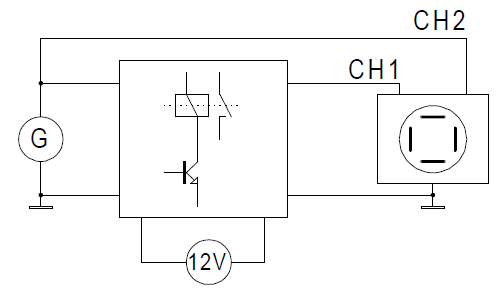
\includegraphics[scale=0.8]{schema.png}
\caption{Schéma zapojení přípravku}
\end{figure}

\section{Naměřené a vypočítané hodnoty}
\begin{table}[H]
\caption{Naměřené hodnoty jednotlivých prvků přípravku}
\begin{tabular}{|c|c|c|c|c|c|c|}
\hline 
Relé & $f\,[Hz]$ & $t_{on}$ & $t_{off}$ & $t_{rise}$ & $t_{fall}$ & Poznámka \\ 
\hline 
Velké relé & 5 & 7,3 ms & 5,9 ms & $<$ 3 us & $<$ 3 us & zákmity \\ 
\hline 
Malé relé & 5 & 4,1 ms & 9,8 ms & $<$ 3 us & $<$ 3 us & zákmity \\ 
\hline 
Jazýčkové relé & 5 & 93,1 us & 75,9 us & $<$ 940 us & 1,4 us & zákmity \\ 
\hline 
Polovodičové relé & 5 & 376 us & 37,5 us & 285 us & 1 us & lineární náběh \\ 
\hline 
Optočlen & 5 & 8,4 us & 10,9 us & 18 us & 19,5 us & exponenciální \\ 
\hline 
Spínací tranzistor & 5 & 16 ns & 100 ns & 24 ns & 185 ns & exponenciální \\ 
\hline 
\end{tabular} 
\end{table}

\section{Závěr}
Z naměřených hodnot lze vyčíst, že se různé prvky velmi zásadně liší. Například čas náběhu $t_{on}$ je u velkého relé $7,3\,ms$ a u spínacího tranzistoru je $t_{on} = 16\,ns$. Obdobně je tomu u vypínacího času. Zajímavé je, že u mechanických relátek dochází k zákmitům. U polovodičového relé dochází k uměle vytvořenému lineárnímu náběhu, aby nedocházelo ke skokové změně a tedy nekonečné časové derivaci.

\section{Přístroje}
\begin{itemize}
\item Napájecí zdroj, evid. 117254
\item Osciliskop DIGI MSO-X2002A, evid. 206127
\item Přípravek se spínači
\end{itemize}

\end{document}
